Postulates of quantum mechanics state, that observable quantities are given by the eigenvalues of the corresponding quantum-mechanical operator. Thus, most quantum mechanics calculations reduce to computing the eigenvalues and eigenfunctions of the operator of interest. The central operator we usually try to find the eigenvalues for is the Hamiltonian $\hat{H}$. The eigenvalues of the Hamiltonian are the energy spectrum that can be measured by, for example, spectroscopic techniques. Part~\ref{part:elstruc} of this book dealt with diagonalization of the Hamiltonian for atoms and molecules, using techniques of \acrfull{tise}. This is the standard approach taken in quantum chemistry. In Chapter~\ref{kap:spec}, we have shown that the energy spectrum can be obtained also from the time evolution of a wave function, which may be often more efficient than the full diagonalization of the Hamiltonian. However, this approach based on the autocorrelation function can provide us only with the eigenvalues, not with the eigenfunctions. Yet the eigenfunctions are necessary to calculate observables of other operators and we often need them. In this Chapter, we will show how both the eigenvalues and eigenfunctions can be obtained from time-dependent techniques using propagation in imaginary time. The imaginary-time propagation is less frequent than the autocorrelation approach and much less frequent than the operator diagonalization, but it is still a useful technique.

\section{*Theoretical background}

In Chapter~\ref{kap:spec}, we have derived an formula for the time evolution of a wave function expressed in the eigenstates of the Hamiltonian operator (see Section~\ref{sec:autocorrintro} and Eq.~\eqref{eq:tdpsi1}):
\begin{equation}
    \psi(x,t) = \sum_k c_k \e^{-\frac{i}{\hbar}E_k t}\phi_k(x) \, ,
    \label{eq:tdpsi2}
\end{equation}
where $E_k$ are the eigenvalues of the Hamiltonian (energies) and $\phi_k(x)$ are its eigenfunctions. The coefficients $c_k$ are constant in time since the Hamiltonian is considered time-independent and are set at time 0. This equation was obtained by applying the propagator $\hat{U}(t)$ to the initial wave function $\psi(x,0)$. 

First, we will inspect the wave function in Eq.~\eqref{eq:tdpsi2}, starting with its norm:
\begin{align}
    \langle\psi(x,t)|\psi(x,t)\rangle &= \sum_k \sum_l c_k^* c_l  \e^{\frac{i}{\hbar}E_k t} \e^{-\frac{i}{\hbar}E_l t} \langle\phi_k(x)|\phi_l(x)\rangle = \sum_k \sum_l c_k^* c_l  \e^{\frac{i}{\hbar}(E_k - E_l) t} \delta_{kl} \notag \\
    &= \sum_k |c_k|^2  \e^{\frac{i}{\hbar}(E_k - E_k) t} =  \sum_k |c_k|^2 = 1 \, .
    \label{eq:itnorm}
\end{align}
As expected, the norm of the wave function is preserved in time since $c_k$s are constant, which is a requirement we have for the wave function in order to conserve the number of particles. The quantity $|c_k|^2$ is the probability of finding state $k$ in a system described by $\psi(x,t)$. In other words, $|c_k|^2$ is the contribution of the $k$-th state to the wave function. Eq.~\eqref{eq:itnorm} shows that all $\phi_k$ contribute constantly the same over time and the composition of the wave function does not vary.\footnote{We remind the reader that the wave function in Eq.~\eqref{eq:tdpsi2} was derived with the assumption of a time-independent Hamiltonian. If the Hamiltonian would depend on time (for example by containing a electromagnetic field), the contributions $|c_k|^2$ would vary.}
Where has the time disappeared in Eq.~\eqrefeq:itnorm} such that the different contributions are constant? The time $t$ appears only in the imaginary exponentials $\e^{\frac{i}{\hbar}E_k t}$ which vanished due to the complex conjugation. 
% The coefficients $c_k$ and eigenfunctions $\phi_k$ left in the expansion are time-independent. Thus, different eigenstates $\phi_k$ contribute to the wave function the same way for all the times. 

Let us now imagine that the state contributions could vary over time. Could we possibly design a propagator, that would enhance the contribution of one of the states and dump the others? If we could achieve this, applying such a propagator would lead to a pure eigenstate $\phi_k$ after the propagation, calculating Hamiltonian eigenstates by means of dynamics instead of solving the \acrlong{tise}. 
Since the time dependence disappears from the norm in Eq.~\eqref{eq:itnorm} due to the complex conjugation, a first natural attempt to create the modified propagator is to replace the complex exponentials with real exponentials. This can be achieved by compounding the imaginary unit $i$ with time $t$, introducing a so-called imaginary time $\tau=it$. The imaginary time is an elusive concept as we have no experience with it in life or even physics. At this point, we will leave the discussion about the concept of imaginary time aside and we ask the reader to view it from a purely mathematical perspective as a new variable $\tau$ introduced into our equations.



Introducing the imaginary time, we can define our new propagator as
\begin{equation}
    \hat{U}_\mathrm{IT}(\tau) = \e^{-\frac{1}{\hbar}\hat{H}(x)\tau} \, .
\end{equation}
The wave function corresponding to $\hat{U}_\mathrm{IT}(\tau)$ is a function of $\tau$ instead of $t$ and reads
\begin{equation}
    \psi(x,\tau) = \sum_k c_k \e^{-\frac{E_k}{\hbar}\tau}\phi_k(x) \, .
\end{equation}
The form the wave function are analogous to the wave function in Eq.~\eqref{eq:tdpsi2} and is derived from the propagator the same way. The expansion coefficients are determined from the initial wave function and also fulfil Eq.~\eqref{eq:initcoeffs}.
Having the wave function, we can again calculate the norm and inspect the state contributions to it:
\begin{align}
    \langle\psi(x,\tau)|\psi(x,\tau)\rangle &= \sum_k \sum_l c_k^* c_l  \e^{-\frac{1}{\hbar}(E_k + E_l) \tau} \langle\phi_k(x)|\phi_l(x)\rangle =\sum_k |c_k|^2  \e^{-2\frac{E_k}{\hbar} \tau} \neq 1 \, .
\end{align}
The state contributions are no longer constant but depend exponentially on the imaginary time as $\e^{-2\frac{E_k}{\hbar} \tau}$. Depending on the sign of the state energy $E_k$, the contribution to the norm decays or increases exponentially. As a result, the norm is not conserved, which means our new propagator is not unitary.

We have now created a propagator which has state contributions varying in time but if we want it to be a useful propagator, we need it to converge to only one of the states. Let us now examine how the state contributions, meaning $|c_k|^2  \e^{-2\frac{E_k}{\hbar} \tau}$, behave with respect to each other. Consider two states $k$ and $l$, where $E_l > E_k$ and $E_l - E_k = \Delta E_{lk} > 0$. The ratio of their contributions to the norm equals to
\begin{equation}
    \frac{|c_k|^2  \e^{-2\frac{E_k}{\hbar}\tau}}{|c_l|^2  \e^{-2\frac{E_l}{\hbar}\tau}} =  \e^{-2\frac{E_k - E_l}{\hbar}\tau} \frac{|c_k|^2}{|c_l|^2}  = \e^{2\frac{\Delta E_{lk}}{\hbar}\tau} \frac{|c_k|^2}{|c_l|^2} \, .
\end{equation}
and shows that the state of lower energy ($k$ in our case) has exponentially increasing contribution compared to the higher energy state $l$. Since this holds for an arbitrary pair of states, the contribution of the lowest energy state to the norm and wave function will be exponentially increasing compared to the other states. As a consequence, the wave function $\psi(x,\tau)$ will converge in the limit of infinite imaginary time to the lowest energy eigenstate $\phi_0$, 
\begin{equation}
    \lim_{\tau\to\infty} \psi(x,\tau) = c_0 \e^{-\frac{E_0}{\hbar}\tau} \phi_0(x) \, ,
\end{equation}
multiplied by $c_0 \e^{-\frac{E_0}{\hbar}\tau}$.

As we have discussed before, the wave function is not normalized but nothing prevents us to renormalize at time $\tau$. We will define a normalized wave function as
\begin{equation}
    \Tilde{\psi} = \frac{\psi(x,\tau)}{\sqrt{\langle\psi(x,\tau | \psi(x,\tau \rangle}}
\end{equation}


 that the exponential in $\tau\to\infty$ goes to zero and our norm also goes to zero (if $E_0 > 0$). 
\begin{equation}
    \lim_{\tau\to\infty} \frac{\psi(x,\tau)}{\sqrt{\langle\psi(x,\tau | \psi(x,\tau \rangle}} = \phi_0(x)
\end{equation}

\begin{figure}[ht!]
    \centering
    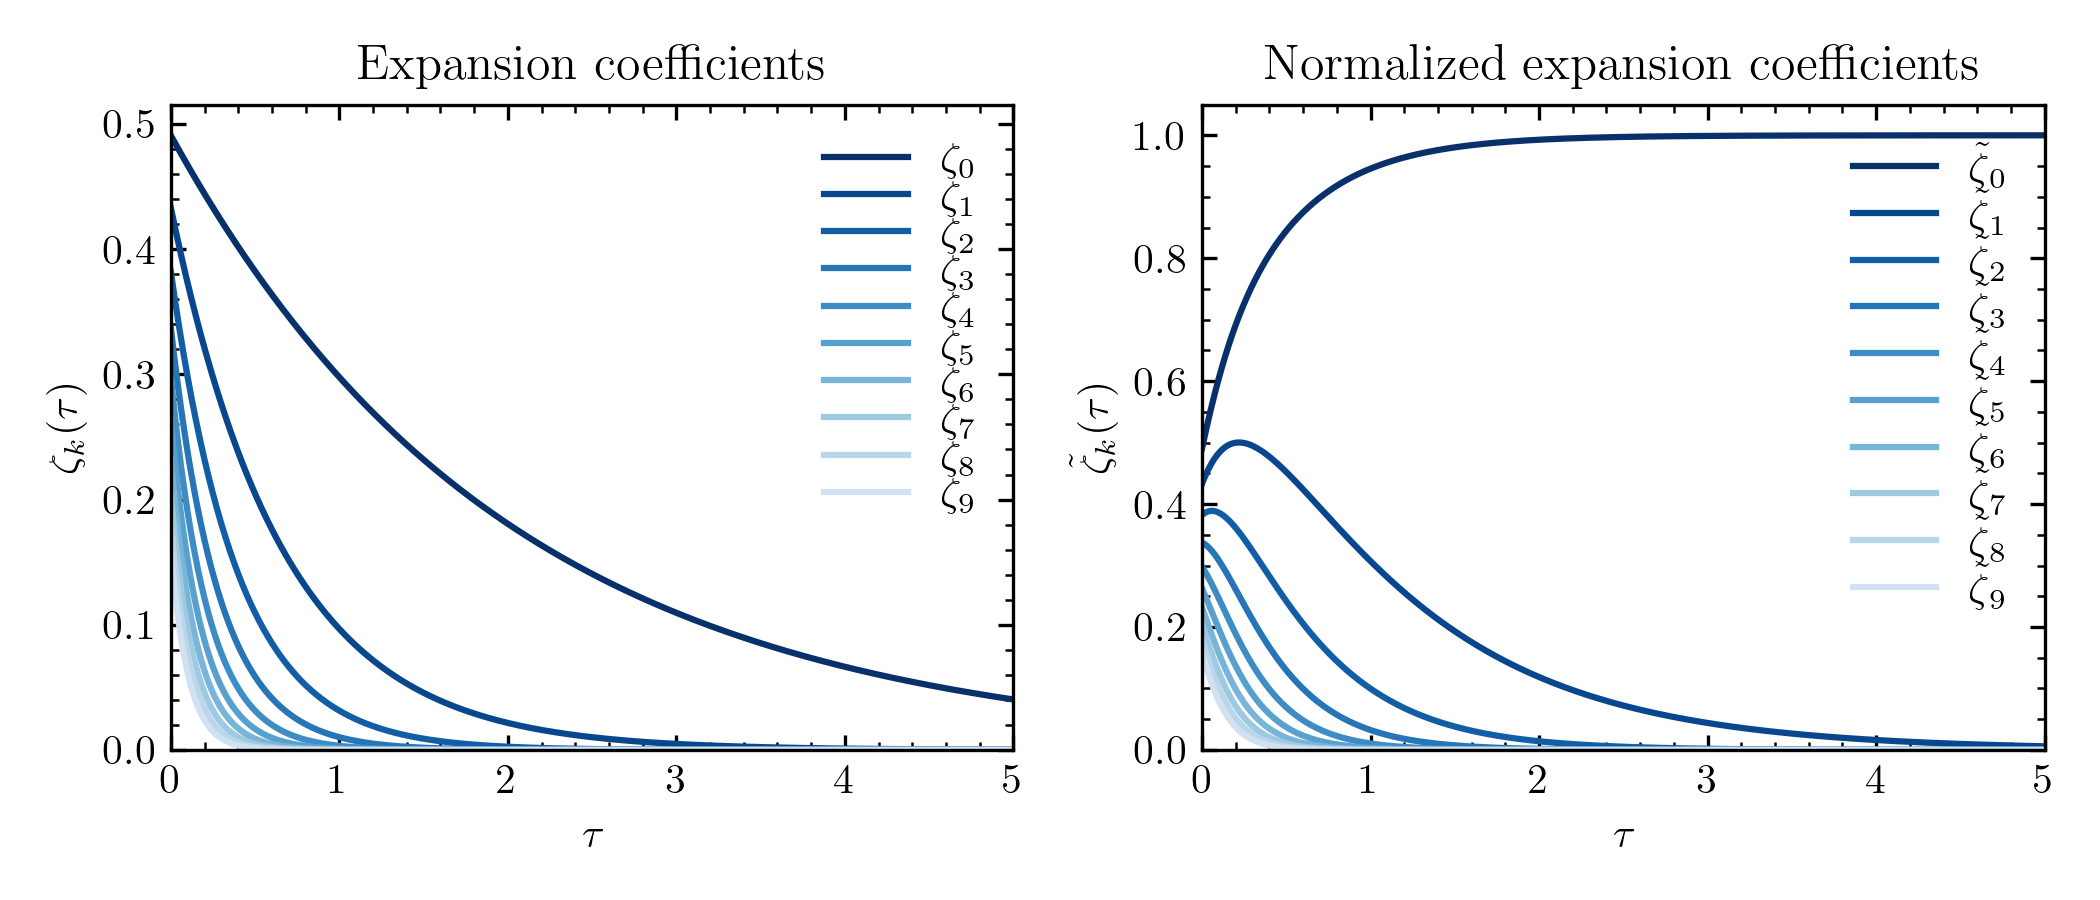
\includegraphics[width=0.9\linewidth]{scriptum/obrazky/itqd/itqd1.png}
    \caption{The imaginary-time evolution of the expansion coefficients $c_i$}
    \label{fig:itqd1}
\end{figure}




\textbf{end}

\vspace{2cm}


\textbf{NOTE ABOUT IT PROPAGATOR}
Let us stop here and discuss the imaginary time. What is it and how should we image a propagation in imaginary time? The concept of imaginary time seems unreal since noone has ever seen watch measuring imaginary time. However, the concept of imaginary time has already been discussed in physics by ..., yet the concept is definitely not easy to grasp. It the imaginary time creates a confusion in the reader, we recommend to look at it from a different point of view. The propagator in imaginary time can be viewed as new operator which, when acting on the wave function, eats the amplitudes of the different energy states such that the lowest energy state is eaten the least. Think about it rather like acting on the wave function by a new operator devised from the real propagator. Note that the imaginary time propagator is not a real propagator because it is not a unitary operator, i.e., it is not perserving norm. The norm in fact exponentially diverges from 1. Yet we still call it IT propagator.

\textbf{next step}

What if we want  different state than the ground state? We have shown previously that the imaginary-time dynamics  converge to the lowest energy state of the initial wave function $\psi(x,0)$.
Thus, the recipe is obvious, we need to project out the lowest energy contribution from the initial wave function, which makes the second lowest state the lowest state.

\begin{equation}
    \Tilde{\psi}(x,0) = \psi(x,0) - c_0 \phi_0(x) = \sum_{k=0}^\infty c_k \phi_k(x) - c_0 \phi_0(x) = \sum_{k=1}^\infty c_k \phi_k(x)
\end{equation}
then
\begin{equation}
    \lim_{\tau\to\infty} \Tilde{\psi}(x,\tau) = c_1  \e^{-\frac{E_1}{\hbar}\tau} \phi_1(x)
\end{equation}

From this, it is obvious, we build the eigenstate from bottom. If we want state m, we need to first obtain all the previous states so that we can project them out. 

Note that we always need to set up the initial wave function $\psi(x,0)$ such that the coefficient of the desired state $k$ is not zero. Then we would not be able to optimize the wave function. Thus, it is usually desirable to construct the wave function such that it breaks the symmetry of the system and contains contributions of all the systems. We can always add some random noise.

\section{*Numerical implementation}

Numerical implementation of the imaginary-time quantum dynamics builds on the real-time quantum dynamics, where the imaginary unit needs to be removed from the exponentials in the propagator. The propagation in time is otherwise the same except for two minor additions to the code.

First, we need to renormalize the propagated wave function $\psi(x,\tau)$ at every time step since we are interested in the normalized $\Tilde{\psi}(x,t)$. The normalization is also important to make the calculation numerically stable. We could propagate $\psi$ without normalization and normalize it at the end, yet we would run into numerical issue soon with the exponential decay or increase of the norm. Plus we still need the norm to evaluate the energy at every step. The renormalization is a simple one-line modification after the propagation step. We can then omit the part of the code checking the norm.

The second addition to the code concerns calculation of excited states (states above the ground state). As we have shown in the previous section, the imaginary-time dynamics converge to the lowest state in the expansion of $\psi(x,0)$. Thus, calculation of an arbitrary state $l$ requires to project out all the states $j$ below $l$ from the initial wave function. Note that the renormalization is necessary after removal of the lower states. Therefore, the renormalization described in the previous paragraph is convenient after this step. The procedure is schematically highlighted in the following scheme:
\begin{equation}
    \psi(x,0) \rightarrow \psi^\prime_l(x,0) = \psi(x,0) - \sum_{j<l}\langle \phi_j | \psi(x,0) \rangle \rightarrow \psi_l(x,0) = \frac{\psi^\prime_l(x,0)}{\langle \psi^\prime_l(x,0) | \psi^\prime_l(x,0) \rangle^2} 
\end{equation}
\textbf{Consider splitting in to equations.}

While this projection of the initial wave function would be in theory sufficient only at the beginning, the numerical precision of a computer alter the wave function a bit at every step which can create a tiny contribution of the lower states. These contributions are at the order of a computer precision, i.e., very small, but they can become important at longer dynamics since they are enhanced exponentially. Hence, the projecting out should be done also during the dynamics. The simplest is to project out at every time step but it is possible to optimize the algorithm and project out with some frequency.

A special  we just need to select the initial wave function such that all the coefficients of the states of interest are non-zero. If the eigenstate we are seeking has $c_k=0$, we will not be able to optimize it with imaginary-time dynamics. This is similar to the previous chapter about the autocorrelation function and we can use the same principles. Contrarily to the real-time quantum dynamics, we need to add two more features.

\section{Code}

\lstset{style=mystyle}
\lstinputlisting[caption=Incomplete code for the imaginary-time quantum dynamics.,language=Python]{codes/exercises/it_quantum_dynamics.py}

\section{Applications}

\subsection*{Exercise: Harmonic oscillator}

The spectrum of a harmonic oscillator was already calculated in the previous chapter as \acrlong{ft} of the autocorrelation function. The same spectrum can be also obtained by the imaginary-time quantum dynamics. Furthermore, the imaginary time dynamics also provide wave functions of the eigenstates which are not available from the autocorrelation function. In this Exercise, we will try to calculate the energies and wave functions of the harmonic oscillator and compare them to the exact analytic results, serving as a validation of the code.

\paragraph{Assignment:} Set up a harmonic oscillator from Eq.~\eqref{eq:qdho} and an initial Gaussian wave packet from Eq.~\eqref{eq:qdgauss} with the following parameters: $m=1$~a.u., $\omega=0.1$~a.u., $x_0=6$~a.u., $p_0=0$~a.u. and $\alpha_0 = 0.3$. Propagate the wave packet in imaginary time to optimise the lowest ten states of the harmonic oscillator. Compare the energies and wave functions with analytic results.

\subsection*{Exercise: Double-well potential}

The double-well potential is one of the simplest model potentials for chemical reactions with an activation barrier. In realistic scenarios, such reactions often exhibit an asymmetry between the two wells, where one minimum is energetically lower than the other. The asymmetric double-well potential can be described by the following expression:
\begin{equation*}
    V(x) = \frac{1}{2}m\omega^2(x^4 - x^2) + \xi x \, .
\end{equation*}
where $m$ is the mass, $\omega$ is the harmonic frequency, and $\xi$ is the asymmetry parameter. This exercise explores the behaviour of wave functions in such a potential, focusing on the number of quantum states localized in the wells and the extent of tunnelling between them.

\paragraph{Assignment:} Prepare a double well potential with parameters $m=20$~a.u., $\omega=2$~a.u. and $\xi=0.5$~a.u. First, initialize the wave function such that it spans both wells and optimize at least fifteen states. 
How many states are located only in one well? Is there a state with energy below the barrier that tunnels between the wells? Can you describe the difference between states below the activation barrier and above it?
Then, initialize the dynamics with a wave function in the form of Eq.~\eqref{eq:qdgauss} and parameters $x_0=-0.90$~a.u., $p_0=0$~a.u. and $\alpha_0 = 2m\omega$~a.u., i.e. the initial wave function will be located in the left well. Observe how the wave function first converges to states in the left well before the lower energy contributions from the right well take over. Can you explain the behaviour?

%%%%%%%%%%%%%%%%%%%%%%%%%% OTHER EXERCISE %%%%%%%%%%%%%%%%%%%%%%%%%%%
%%%%%%%%%%%%%%%%%%%%%%%%%% TO BE FINISHED %%%%%%%%%%%%%%%%%%%%%%%%%%%

% \subsection*{*Exercise: Morse potential}

% \begin{equation*}
%     V(x) = D_e \left(1 - \e^{-a(x-x_e)}\right)^2 \, .
% \end{equation*}

% \paragraph{Assignment:} Text

% \subsection*{*Exercise: OH radical}

% % Maybe OH radical? What temperature would lead to Boltzmann population of the most loosely bound state to be 0.2%?

% \paragraph{Assignment:} Text